\documentclass[a4paper, fleqn]{article}
\usepackage{enumitem}
\usepackage{amsmath, amssymb}
\usepackage{xstring}
\usepackage{graphicx} % For including figures
\graphicspath{{./figs/}} % Path to figures
\usepackage[labelformat=empty]{caption}
% Set engineering notation
\providecommand{\sci}[1]{\protect\ensuremath{\times 10^{\StrSubstitute[0]{#1}{e}{}}}}
\setlength{\parindent}{0pt} % Set paragraph indentation to zero

\begin{document}

\underline{\textbf{\large Tutorial 2: Power Screw}}
\vspace{10pt}

\section*{In-class activity}

A screw of M10x1.5 is used as a lead screw for a machine with a torque of 10 Nm travelled linearly at 10mm/s. Determine;
\begin{enumerate}[label=(\roman*)]
    \item the mean diameter of the screw.
    \item angular speed of the screw in rpm.
    \item power carried by the screw.
\end{enumerate}

\textbf{Example Solution}

\begin{enumerate}[label=(\roman*)]
    \item Mean diameter of the screw:
    \begin{equation*}
        \begin{aligned}
        d_m = \frac{D + (D - p)}{2} = \frac{10 + (10 - 1.5)}{2} = 9.25 \text{ mm}
        \end{aligned}
    \end{equation*}

    \item Angular speed of the screw in rpm:
    \begin{equation*}
        \begin{aligned}
        V_{linear} &=Lead \times n_{rpm} \times \frac {1 min}{60 s} \\
        \frac {10mm}{1s} &=\frac {1.5mm}{1 rev} \times n_{rpm} \times \frac {1 min}{60 s} \\
        n_{rpm} &= 400rpm
        \end{aligned}
    \end{equation*}

    \item Power carried by the screw:
    \begin{equation*}
        \begin{aligned}
        P &= \omega T=  \frac{2\pi n}{60} T\\
        &= \frac{2\pi (400)}{60} (10)\\
        &= 418.88 W
        \end{aligned}
    \end{equation*}
\end{enumerate}

\section*{Theory}

\begin{enumerate}
    \item What is a power screw?
    \item What is the purpose of a power screw?
    \item Draw and make a detail sketch of a square thread, Acme and Modified thread. Explain the difference between these threads and its applications.
\end{enumerate}

\newpage
\section*{Calculations}
\vspace{10pt}

\textbf{Question 1}

A screw jack has a triple threaded Acme power screw of M30x4, is used to lift a load of a 6kN. Determine;

\begin{enumerate}[label=(\roman*)]
    \item The screw lead, mean diameter and helix angle
    \item The screw torque required to move the load up
    \item Is the screw overhauling
    \item The efficiency of the jack, if collar friction is used
    \item The length of a crank required if F=150N is exerted by an operator
\end{enumerate}

Given: f=0.12, fc=0.09 and dc=40mm

\vspace{10pt}
\textbf{Example Solution}
\vspace{10pt}

$n = 3$(triple thread)\\
$\alpha = 14.5$ (Acme thread)\\
$diameter,D = 30mm$\\
$pitch,p = 4$\\
$Load = 6000N$\\
$f = 0.12$\\
$f_c = 0.09$\\
$d_c = 40mm$\\
\vspace{10pt}

i-Find lead first,
\begin{equation*}
    \begin{aligned}
    Lead, L &=np\\
    &=3\times4mm = 12mm/turn    
    \end{aligned}
\end{equation*}

Find mean diameter,
\begin{equation*}
    \begin{aligned}
    d_m &= \frac {D+(D-p)}{2}\\  
    &= \frac {30+(30-4)}{2}\\ 
    &= 28mm
    \end{aligned}
\end{equation*}

Find helix angle,
\begin{equation*}
    \begin{aligned}
    \tan\lambda &= \frac{L}{\pi d_m}\\
    &= \frac{12mm}{\pi 28mm} \\
    &=0.136\\
    \lambda &= \tan^{-1}(0.136)\\
    &=7.768^{\circ}
    \end{aligned}
\end{equation*}

ii-Find torque to lift the load,
\begin{equation*}
    \begin{aligned}
    T_u = \frac{Wd_m}{2} \frac{f+\cos\alpha_n \tan\lambda}{\cos\alpha_n + f\tan\lambda} + \frac{Wf_c d_c}{2}
    \end{aligned}
\end{equation*}

Find $\alpha_n$
\begin{equation*}
    \begin{aligned}
    \tan \alpha_n &= \cos \lambda \tan \alpha\\
     &= \cos 7.768 \tan 14.5\\
    &= 14.37^{\circ}
    \end{aligned}
\end{equation*}

Substitute known values into torque to lift the load equation,
\begin{equation*}
    \begin{aligned}
    T_u &= \frac{Wd_m}{2} \frac{f+\cos\alpha_n \tan\lambda}{\cos\alpha_n + f\tan\lambda} + \frac{Wf_c d_c}{2} \\
    &= \frac{6000(28\sci{e-3})}{2} \times\frac{0.12+\cos(14.37) \tan(7.768)}{\cos(14.37) - 0.12\tan(7.768)} + \frac{6000(0.09)(40\sci{e-3})}{2} \\
    &= 33 kN
    \end{aligned}
\end{equation*}

iii-Check if the screw is overhauling,

Screw overhaul when,
\begin{equation*}
    \begin{aligned}
    f &\le \cos \alpha_n \tan \lambda \\
    0.12 &\le \cos(14.37) \tan(7.768)\\
    0.12 &\le 0.136\\
    \end{aligned}
\end{equation*}

$\cos \alpha_n \tan \lambda$ is greater than $f$, therefore the screw is overhauling.
\vspace{10pt}

OR, can check using torque to lower the load. \\
If the value is negative, it will overhaul.
$$T_d = \frac{Wd_m}{2} \frac{f-\cos\alpha_n \tan\lambda}{\cos\alpha_n + f\tan\lambda} + \frac{Wf_c d_c}{2}$$

$T_d=-1.02kN$, which is negative, therefore the screw is overhauling.
\vspace{10pt}

iv- Find efficiency of the jack, if collar friction is used,
\begin{equation*}
    \begin{aligned}
    e &=\frac{d_m \tan \lambda}{d_m \frac{f+\cos\alpha_n \tan\lambda}{\cos\alpha_n - f\tan\lambda}+d_c f_c} \\
    &=\frac{28\sci{e-3} \tan(7.768)}{28\sci{e-3} \frac{0.12+\cos(14.37) \tan(7.768)}{\cos(14.37) - 0.12\tan(7.768)}+40\sci{e-3} (0.09)} \\
    &=0.47
    \end{aligned}
\end{equation*}

v- Find the length of a crank required if F=150N is exerted by an operator,
\begin{equation*}
    \begin{aligned}
    T_u &= F \cdot r\\
    33\sci{e3} &= 150 \cdot r\\
    r &= \frac{33\sci{e3}}{150}\\
    &= 0.22 m
    \end{aligned}
\end{equation*}

\newpage
\textbf{Question 2}

\begin{figure}[h]
    \centering
    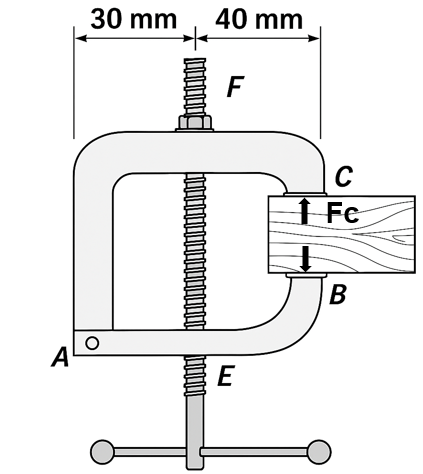
\includegraphics[width=0.5\textwidth]{t2-q2.png}
    \caption{Figure Q2}
\end{figure}

The clamp assembly as shown in Figure Q2 consists of member AB and AC, which are pin connected at A. The clamp works by rotating a single start ACME thread $(\alpha=14.5^{\circ})$ with the size of 12.5 mm and pitch of 2.5 mm. At this instant, the compressive force, Fc on the wood between B and C is 180 N. The collar at the assembly has a mean diameter of 13.5 mm. Assume all the friction coefficient between all surface contracts is 0.3. Determine:

\begin{enumerate}[label=(\roman*)]
    \item the load acting at the screw.

    \item the torque required to tighten the screw.

    \item the maximum compressive force, Fc, if allowable normal stress at the screw is 10 MPa.
\end{enumerate}


\newpage

\textbf{Question 3}

The bench hold-down clamp is being used to clamp two boards together while they are being glued as shown in Figure Q3. The clamp consists of a screw having single square threads of M12 X 2 and coefficient of friction in the screw thread is taken as 0.2. The screw producing maximum power of 35 W when moving at 2mm/s axially.

\begin{enumerate}[label=(\roman*)]
    \item the torque acting at the screw

    \item the compression force exerted on the boards when torque as (i) is applied

    \item Recommend the suitable handle length, d if the compression force is increased to 1.5 kN, thus the user need to apply force of 100 N on the handle.
\end{enumerate}

\begin{figure}[h]
    \centering
    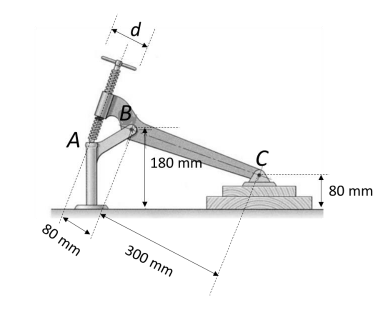
\includegraphics[width=0.5\textwidth]{t2-q3.png}
    \caption{Figure Q3}
\end{figure}


\newpage
\textbf{Question 4}

The screw is a double-start ACME thread of M12x 1.5. The clamping force exerted at G is FG=900 N. The mean diameter of the collar is dc = 22 mm. Coefficients of friction for screw and collar are estimated as f = 0.3 and fc = 0.15 respectively. The screw will travel axially at 95 mm/s. Find,

\begin{enumerate}[label=(\roman*)]
\item The screw lead, mean diameter, and helix angle
\item The force and axial stress acting on the screw
\item The torque for lifting and for lowering the load
\item The force needed to apply perpendicular at E to produce the clamping force
\item The angular rotation of the screw in rpm
\item The power produced by the power screw
\item The efficiency of the jack when lifting the load
\item Whether the screw is overhauling
\item Determine the maximum compressive force, if the new allowable normal stress at thescrew is 30 MPa.
\item Recommend the suitable length of the handle if the compression force is increased to1.5 kN, thus the user needs to apply force of 100 N on the handle.
\item Determine the new efficiency on the screw if a SQUARE thread is used. Compare theefficiency.
\end{enumerate}

\begin{figure}[h]
    \centering
    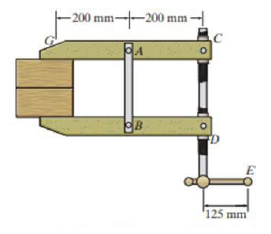
\includegraphics[width=0.5\textwidth]{t2-q4.png}
    \caption{Figure Q4}
\end{figure}

\newpage

\textbf{Answer}
\vspace{10pt}

\textbf{Q2}

i- Load acting at the screw, $F_E=420N$

ii- Torque required to tighten the screw, $T=1.77Nm$

iii- Maximum compressive force, $F_c=336.6N$

\vspace{10pt}
\textbf{Q3}

i- Torque acting at the screw, $T=1.67Nm$

ii- Compression force exerted on the boards, $F_c=420N$

iii- Suitable handle length, $d=0.25m$

\vspace{10pt}
\textbf{Q4}

i- Screw lead, $L=3mm$, mean diameter, $d_m=10.5mm$ and helix angle, $\lambda=8.21^{\circ}$

ii- Force acting on the screw, $F=1088.9N$ and axial stress, $\sigma=12.47MPa$

iii- Torque for lifting, $T_u=2.98Nm$ and for lowering the load, $T_d=-0.48Nm$

iv- Force needed to apply perpendicular at E, $F=29.8N$

v- Angular rotation of the screw, $n=3030rpm$

vi- Power produced by the power screw, $P=94.8W$

vii- Efficiency of the jack when lifting the load, $e=0.36$

viii- The screw is overhauling

\vspace{10pt}
Well-defined Problem

ix- Maximum compressive force, $F_c=2412N$

x- Suitable length of the handle, $d=0.3m$

xi- New efficiency on the screw if a SQUARE thread is used, $e=0.44$. The efficiency is increased by 0.08 or 8\%.

\end{document}